Considerando os 3 elementos (A, B e C) indicados na tabela periódica abaixo, determine:

\begin{center}
	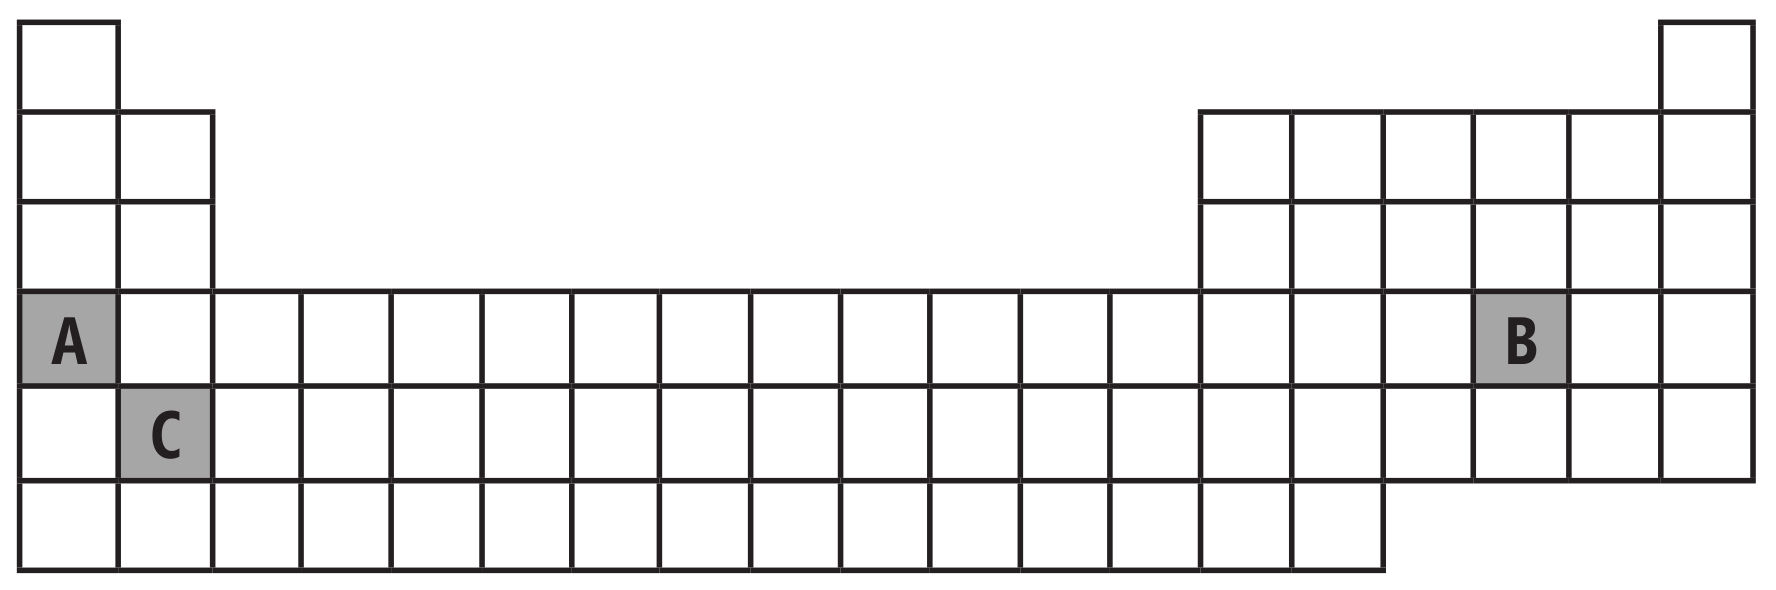
\includegraphics[width = 0.8\textwidth]{figure.png}
\end{center}

\begin{enumerate}[label = (\alph*)]
	\item o átomo que apresenta:
		\begin{enumerate}[label = (a.\roman*)]
			\item o maior raio atômico.
			\item a maior afinidade eletrônica.
			\item a maior energia de ionização.
		\end{enumerate}
	\item a fórmula do composto formado entre:
		\begin{enumerate}[label = (b.\roman*)]
			\item o átomo A e o átomo B.
			\item o átomo B e o flúor.
			\item o átomo C e o oxigênio.
		\end{enumerate}
\end{enumerate}
